% !TeX spellcheck = ru_RU
% !TEX root = vkr.tex

\section{Эксперимент}

\subsection{Условия эксперимента}

Экспериментальное исследование проводилось на трёх аппаратных платформах: двух одноплатных компьютерах на базе архитектуры RISC-V (Banana Pi BPI-F3 и StarFive VisionFive 2) и одной референсной платформе на базе архитектуры x86-64 со встроенной графикой Intel (Intel Core i9-12900H с Intel Iris Xe Graphics).

Характеристики платформ подробно описаны в разделе~2.4. Кратко:
\begin{itemize}
    \item \textbf{Banana Pi BPI-F3}: SpacemiT K1 (8 ядер RISC-V @ 2.0 ГГц), IMG BXE-2-32 GPU, 16 ГБ LPDDR4-2666;
    \item \textbf{StarFive VisionFive 2}: JH7110 (4 ядра RISC-V @ 1.5 ГГц), IMG BXE-4-32 MC1 GPU, 8 ГБ LPDDR4-2800;
    \item \textbf{Intel Iris Xe}: Intel Core i9-12900H (14 ядер @ до 5.0 ГГц), Intel Iris Xe Graphics (96 EU), 24 ГБ DDR5-4800.
\end{itemize}

Для каждой конфигурации параметров и каждого ядра выполнялось по 100 прогонов операции умножения матриц. Измерялось только время выполнения OpenCL ядра, без учёта времени на подготовку данных, их копирование в память устройства и обратно. Это позволило получить чистую оценку вычислительной производительности различных реализаций алгоритма. Для обработки результатов использовалось среднее арифметическое значение времени выполнения.

Для обеспечения стабильности измерений на RISC-V платформах использовалось пассивное охлаждение, частоты процессоров работали в штатном режиме с динамическим управлением. Скрипты для автоматизации тестирования и обработки результатов доступны в форке репозитория MyGEMM~\cite{mygemm_repo_test}.

\subsection{Тестовые данные}

В качестве тестовых данных использовались квадратные матрицы размером $1024 \times 1024$ элементов типа \texttt{float} (32-бит). Размер матриц был выбран достаточно большим для выявления различий в производительности различных оптимизаций, но при этом умещающимся в память всех тестируемых устройств.

Тестировались 11 ядер библиотеки MyGEMM (от наивной реализации до продвинутых оптимизаций) с различными наборами параметров конфигурации. Для ядер 1--3 варьировался параметр TS (Tile Size) со значениями из множества \{8, 16\}. Попытки запуска с TS=32 приводили к ошибке выполнения ``Invalid work group size''.

Для ядер 4--10 тестировались комбинации параметров TSM и TSN из множества \{32, 64, 128\} с соответствующими значениями WPTM и WPTN, что дало 9 уникальных конфигураций для каждого ядра. Ядро 11 имеет фиксированную конфигурацию параметров, определённую реализацией clBLAS.

Все конфигурации параметров были подобраны с учётом ограничения максимального размера рабочей группы в 32 потока на RISC-V платформах.

\subsection{Результаты измерений}

Результаты экспериментов представлены на рисунках~\ref{fig:perf_bananapi}--\ref{fig:perf_intelxe} для каждой из тестируемых платформ. На графиках показано среднее время выполнения операции умножения матриц в секундах для различных ядер и конфигураций параметров.

\begin{figure}[H]
\centering
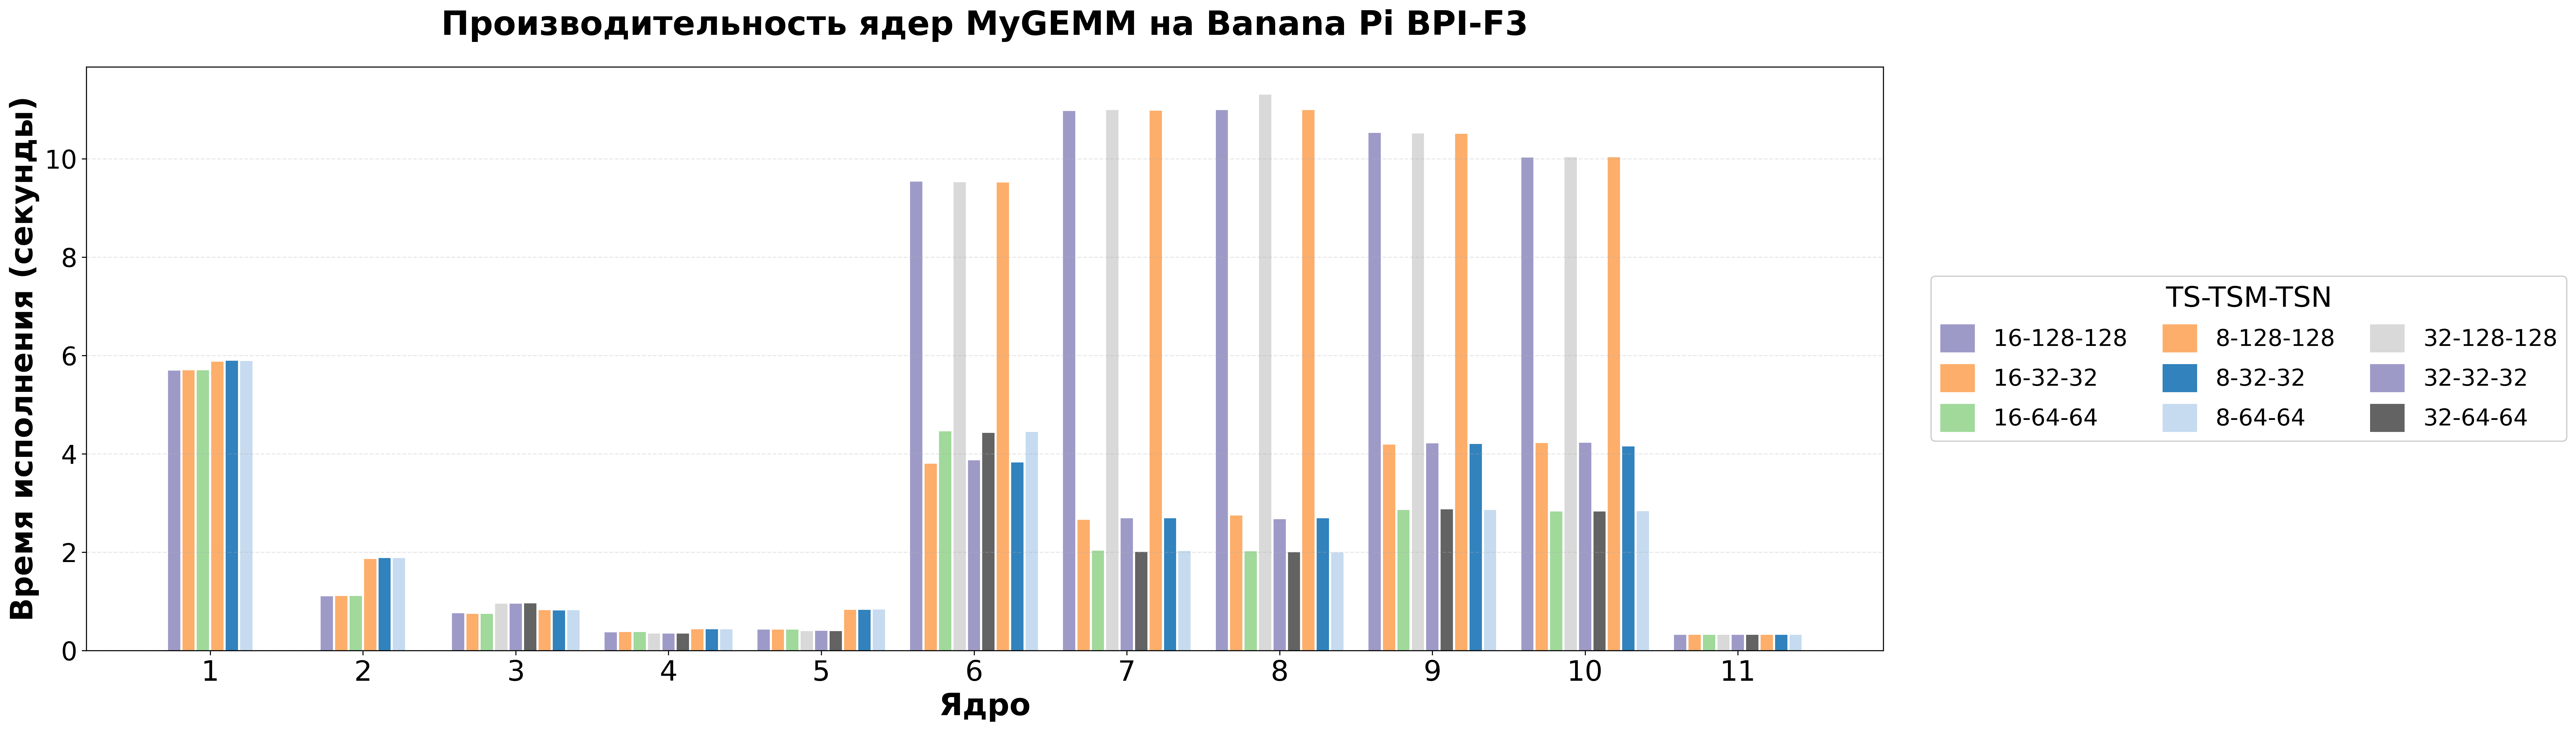
\includegraphics[width=1\textwidth]{figures/banana_pi.png}
\caption{Производительность ядер MyGEMM на платформе Banana Pi BPI-F3}
\label{fig:perf_bananapi}
\end{figure}

\begin{figure}[H]
\centering
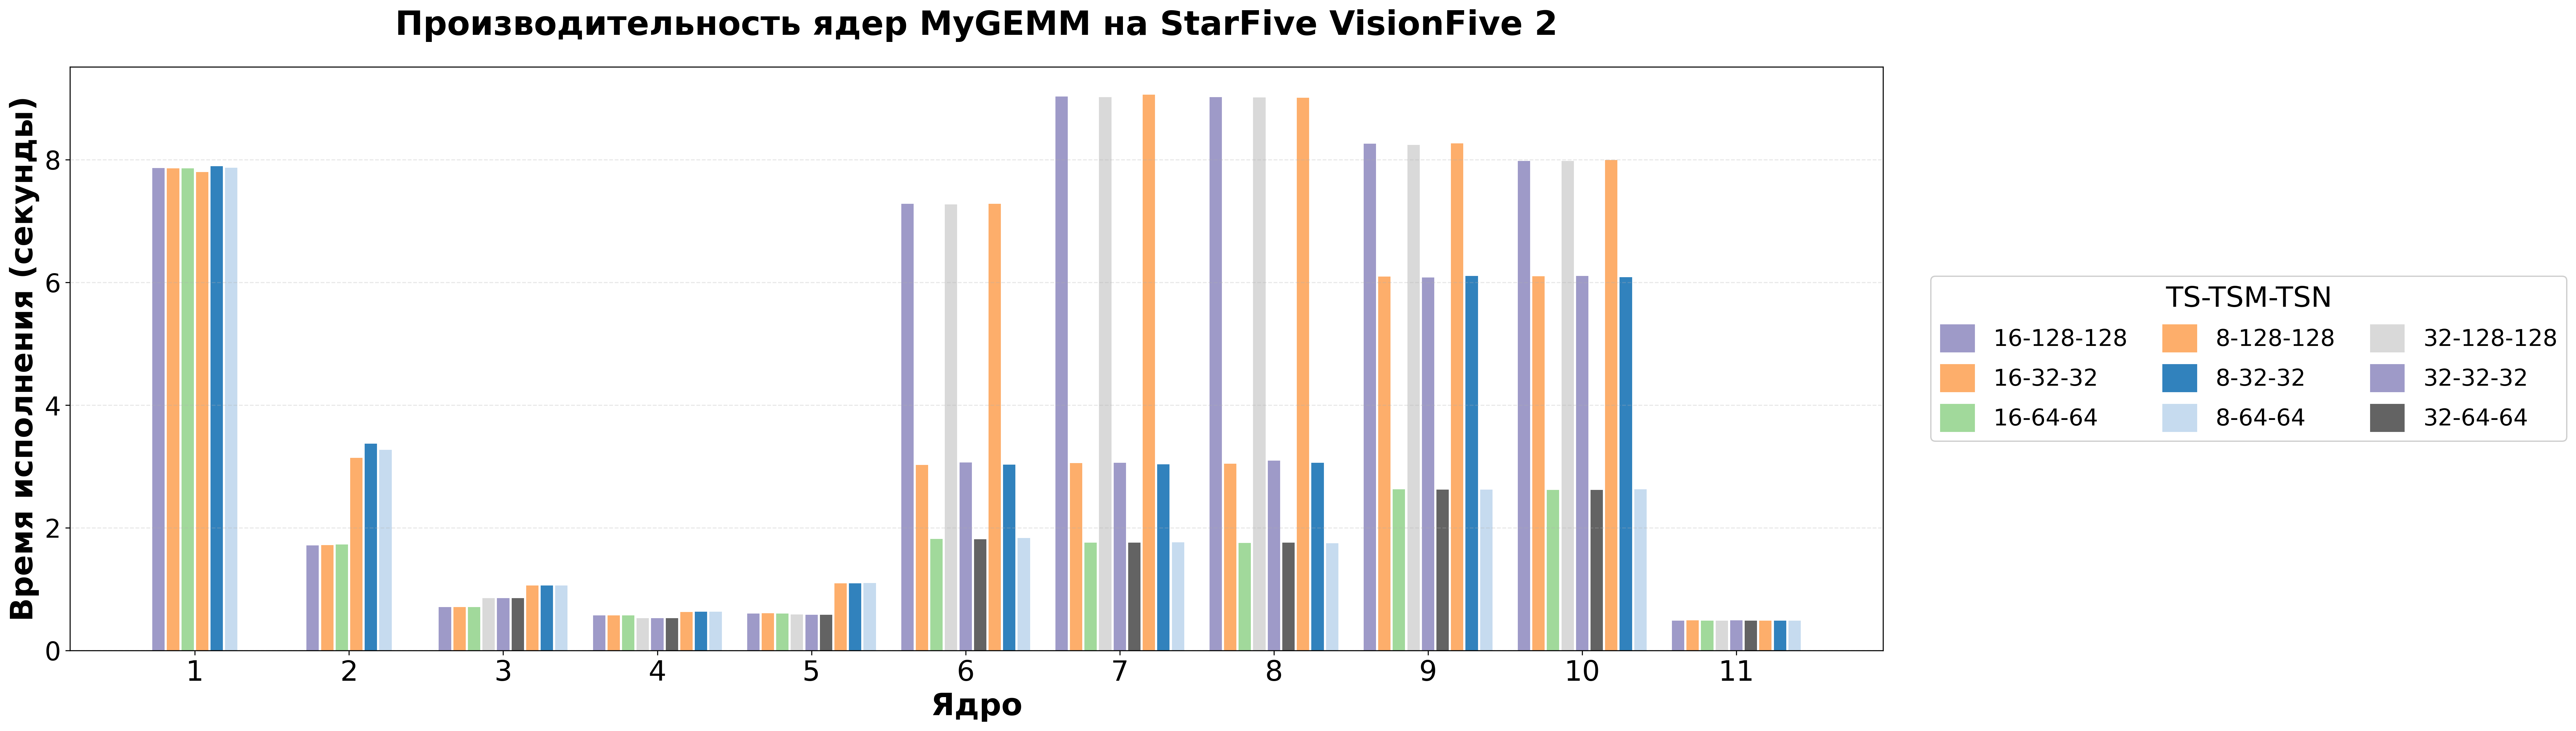
\includegraphics[width=1\textwidth]{figures/starfive.png}
\caption{Производительность ядер MyGEMM на платформе StarFive VisionFive 2}
\label{fig:perf_starfive}
\end{figure}

\begin{figure}[H]
\centering
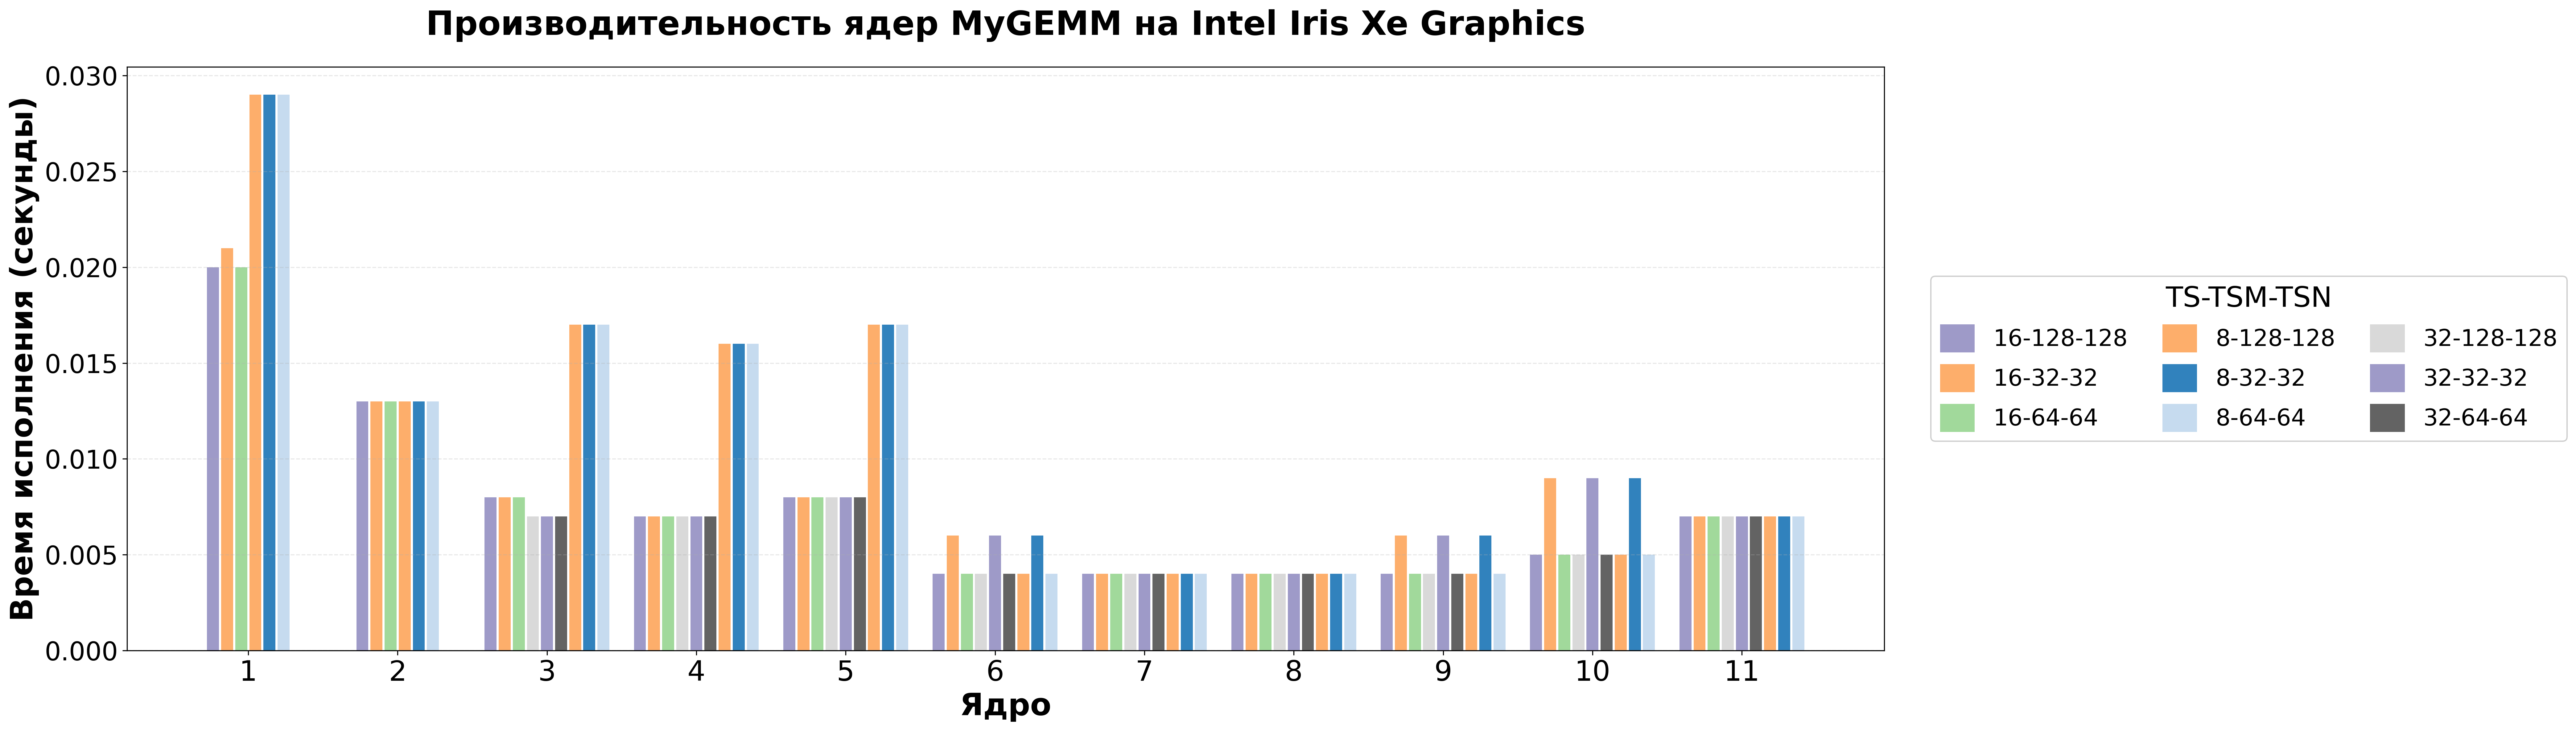
\includegraphics[width=1\textwidth]{figures/intel_xe.png}
\caption{Производительность ядер MyGEMM на референсной платформе Intel Iris Xe}
\label{fig:perf_intelxe}
\end{figure}

\subsubsection{Анализ результатов}

Экспериментальные данные демонстрируют значительные различия в производительности между RISC-V платформами и референсной системой Intel Iris Xe. Референсная платформа показывает время выполнения в диапазоне 0.004--0.029 секунд для различных ядер, что в среднем в 200--400 раз быстрее, чем RISC-V платформы.

Среди RISC-V платформ Banana Pi BPI-F3 демонстрирует лучшую производительность по сравнению со StarFive VisionFive 2, что объясняется более высокой тактовой частотой (2.0 ГГц против 1.5 ГГц) и большим количеством вычислительных ядер (8 против 4). Среднее время выполнения на Banana Pi составляет 0.3--11 секунд, на StarFive -- 0.5--9 секунд. В среднем Banana Pi опережает StarFive в 1.3--1.5 раза в зависимости от ядра.

Ключевые наблюдения по результатам экспериментов:

\textbf{Наилучший результат.} Ядро 11 (clBLAS-подход) демонстрирует наилучшую производительность на всех трёх платформах. На Banana Pi время выполнения составляет 0.32 сек (ускорение в 18.4 раза относительно наивной реализации), на StarFive -- 0.49 сек (ускорение в 16.1 раз), на Intel Iris Xe -- 0.007 сек. Это ядро не использует локальную память и полностью полагается на регистровую блокировку с векторными типами данных. Стабильность результатов ядра 11 на RISC-V платформах (время практически не зависит от параметров конфигурации) указывает на хорошую оптимизацию под архитектурные особенности этих процессоров.

\textbf{Проблемы векторизации.} Ядра 6--10, активно использующие векторизацию загрузки и записи данных, показывают неожиданно низкую производительность на RISC-V платформах. Время выполнения достигает 9--11 секунд на Banana Pi и 7--9 секунд на StarFive, что в 10--30 раз медленнее более простых ядер 3--5. При этом на Intel Iris Xe эти же ядра демонстрируют отличные результаты (0.004--0.009 сек). Разница в производительности между RISC-V и Intel для векторизованных ядер составляет 600--1000 раз, что указывает на серьёзные проблемы с реализацией векторных операций в драйверах OpenCL для архитектуры RISC-V.

\textbf{Эффективность базовых оптимизаций.} Ядра 2--5, использующие блочную обработку с локальной памятью и work-per-thread оптимизацию, показывают хороший результат. Ядра 4 и 5 (2D регистровая блокировка с транспонированием) достигают времени 0.3--0.6 секунд на RISC-V платформах, что в 10--25 раз быстрее наивной реализации (ядро 1). Эти результаты демонстрируют, что классические оптимизации для GPU эффективно работают и на встроенных графических ядрах RISC-V процессоров.

\textbf{Влияние параметров конфигурации.} Анализ графиков показывает, что для ядер 1--3 изменение параметров TSM и TSN практически не влияет на производительность, поскольку эти ядра используют только параметр TS для определения размера рабочей группы. Для ядер 4--10 наблюдается заметная зависимость от конфигурации: увеличение TSM и TSN при фиксированном TS обычно не приводит к значительному изменению производительности, что объясняется ограничениями локальной памяти и аппаратными лимитами на размер рабочих групп.

\textbf{Ограничения архитектуры.} Жёсткое ограничение размера рабочей группы в 32 потока на RISC-V платформах существенно ограничивает возможности оптимизации. Многие конфигурации параметров, эффективные на дискретных GPU (где размер рабочей группы может достигать 1024 потоков), не могут быть использованы на RISC-V. Это особенно заметно для ядер 6--10, которые были оптимизированы для больших рабочих групп.

Результаты показывают, что для достижения приемлемой производительности на RISC-V платформах следует отдавать предпочтение подходу, реализованному в ядре 11 (clBLAS), который не использует локальную память и основывается на регистровой блокировке. Ядра с активной векторизацией (6--10) следует избегать до улучшения драйверов OpenCL. Классические оптимизации с использованием локальной памяти (ядра 2--5) обеспечивают приемлемое ускорение и могут использоваться как компромиссное решение.

\textbf{Техническое объяснение провала векторизации.} Анализ архитектуры и особенностей драйверов позволяет сформулировать обоснованную гипотезу о причинах катастрофически низкой производительности векторизованных ядер 6--10 на RISC-V платформах.

Ключевое различие между ядрами 6--10 и ядром 11 заключается не в использовании векторных типов данных (оба подхода их применяют), а в способе доступа к памяти. Ядра 6--10 активно используют векторизованные операции загрузки и записи OpenCL (\texttt{vload2}, \texttt{vload4}, \texttt{vload8}, \texttt{vstore2}, \texttt{vstore4}, \texttt{vstore8}), которые должны обеспечивать эффективную пакетную передачу данных между глобальной памятью и регистрами. Ядро 11, напротив, использует векторные типы данных (\texttt{float4}, \texttt{float8}) для вычислений, но загружает данные через обычные скалярные операции с последующей упаковкой в векторные регистры.

Согласно документации Imagination Technologies~\cite{img_opencl}, графические ядра PowerVR Rogue оптимизированы для операций над данными типа \texttt{float} и могут выполнять до двух операций с плавающей точкой за такт на один поток. Архитектура организует потоки в группы до 32 (warps), что совпадает с аппаратным ограничением на размер рабочих групп на тестируемых RISC-V платформах. Однако эффективная работа векторных операций загрузки и записи требует:
\begin{itemize}
    \item правильного выравнивания данных в памяти (alignment);
    \item оптимизированных аппаратных путей доступа к памяти для пакетных операций;
    \item корректной компиляции векторных инструкций OpenCL в команды GPU.
\end{itemize}

Драйверы OpenCL для PowerVR BXE на RISC-V платформах находятся на ранних стадиях разработки. Сообщество разработчиков сообщает о множественных проблемах с драйверами BXE, включая артефакты рендеринга и нестабильную работу~\cite{img_opencl}. Открытый драйвер Mesa для PowerVR пока не полностью поддерживает архитектуру BXE и имеет статус ``частично поддерживаемой'' без активной разработки.

Наиболее вероятные причины деградации производительности векторизованных ядер:

\textbf{1. Неоптимизированная компиляция векторных операций.} Компилятор OpenCL может некорректно транслировать векторные операции \texttt{vload}/\texttt{vstore} в команды GPU, приводя к их декомпозиции на последовательность скалярных операций. Вместо одной векторной загрузки \texttt{vload8} выполняется 8 отдельных скалярных загрузок, что полностью нивелирует преимущества векторизации и добавляет накладные расходы.

\textbf{2. Эмуляция векторных операций на CPU.} В отсутствие надлежащей поддержки векторных операций в драйвере, они могут частично или полностью эмулироваться на стороне CPU, что объясняет 600--1000-кратную деградацию производительности. При этом данные копируются из памяти GPU в память CPU, обрабатываются на CPU и копируются обратно, что создаёт огромные накладные расходы на передачу данных.

\textbf{3. Проблемы с выравниванием и кэшированием.} PowerVR архитектура критична к выравниванию данных в памяти для эффективной работы векторных операций. Некорректная обработка выравнивания в драйвере может приводить к неэффективным паттернам доступа к памяти, промахам кэша и дополнительным операциям выравнивания.

Успешная работа ядра 11 подтверждает гипотезу: это ядро избегает проблемных векторных операций загрузки/записи, используя вместо них прямую работу с регистрами и стандартные операции доступа к памяти. Такой подход обходит недостатки реализации векторизации в драйвере, сохраняя при этом преимущества векторных вычислений на аппаратном уровне.

Для подтверждения этой гипотезы необходимо профилирование выполнения ядер с использованием инструментов анализа производительности OpenCL и исследование промежуточного представления (IR) компилятора, что выходит за рамки данной работы, но является важным направлением будущих исследований.